% !TeX root = 00_main.tex

\chapter[Experimental Evaluation]{Experimental Evaluation}
\label{sec:experiments}

The proposed approach is evaluated on a dataset mined from Twitter using their public API, feeding from a global $1\%$-sample over the time interval from December 30, 2013 to March 24, 2014, using a $(51.25,51.75)$ degrees longitude to $(-0.55,0.30)$ degrees latitude window covering the London region shown in Figure \ref{fig:intro:10user}.

\begin{figure}[ph]
	\centering
	\begin{subfigure}[b]{\textwidth}
		\centering
		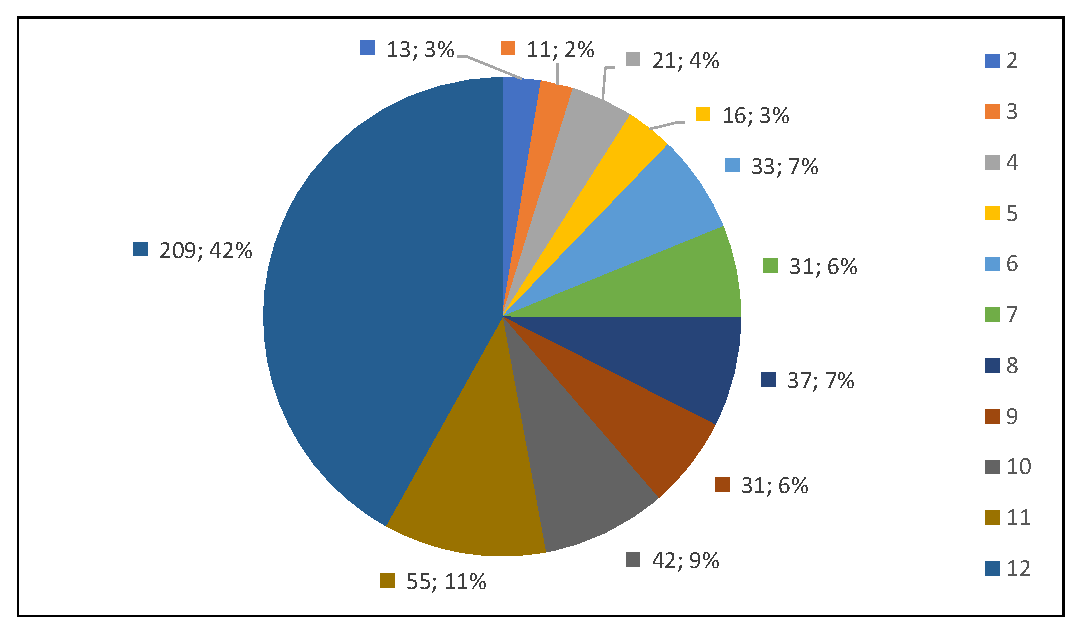
\includegraphics[width = 0.8\textwidth]{figures/500_trajectories_per_user}
    \subcaption{Trajectories within the 12 epochs}
    \label{fig:500_traj}
	\end{subfigure}

	\begin{subfigure}[b]{\textwidth}
		\centering
		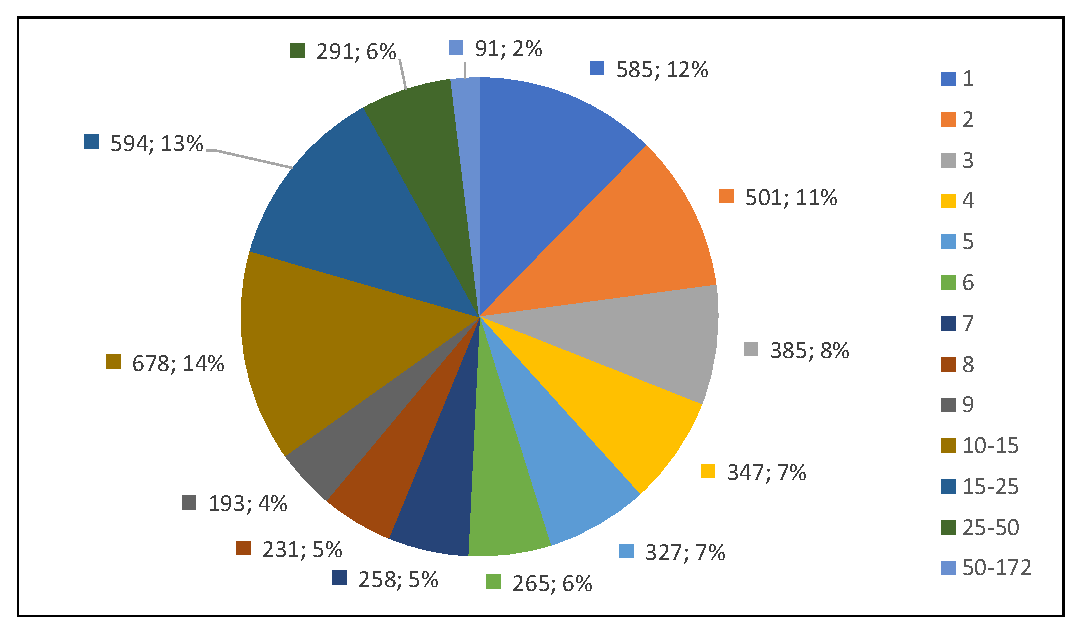
\includegraphics[width = 0.8\textwidth]{figures/500_observations_per_trajectory}
		\subcaption{Observations per one-week Trajectory}
    \label{fig:500_obs}
	\end{subfigure}
  \caption{Distribution of the Top 500 most prolific users in the London-Twitter Dataset.}\vspace{-0.2cm}
  \label{fig:500_dist}
	\figSpace
\end{figure}

Out of these London-Tweets, the top-500 most prolific users were selected, excluding obvious spammer or bot users. This dataset is split into temporal epochs of one-week. Thus, the database contains a total of $|\mathcal{U}|=500$ users, and a total of $|\mathcal{E}|=12$ epochs. Consequently, the database $\DB$ contains a total of $\mathcal{U}\times\mathcal{E}=6000$ trajectories.

To discretize space, a spatial grid is applied on the aforementioned rectangle covering the London region, having an extent $ext$ in longitude and latitude ranging from $0.01'$ to $0.001'$. The set of all resulting grid cells constitutes the set of spatial regions $\mathcal{S}$, having $|\mathcal{S}|=4.250$ cells for $ext=0.01'$ and $425.000$ cells for $ext=0.001'$. Table \ref{} shows all grid sizes as well as the dimensions of the related trajectories.

\begin{table}
  \centering
  \caption{Grid Sizes and Total Cells}
  \begin{tabular}{|l|l|l|l|}
    \hline
		{\bf Degrees} & {\bf X Size} & {\bf Y Size} & {\bf Total} \\\hline
		0.010 & 85 & 50 & 4,250 \\\hline
		0.009 & 95 & 56 & 5,320 \\\hline
		0.008 & 107 & 63 & 6,741 \\\hline
		0.007 & 122 & 72 & 8,784 \\\hline
		0.006 & 142 & 84 & 11,928 \\\hline
		0.005 & 170 & 100 & 17,000 \\\hline
		0.004 & 213 & 125 & 26,625 \\\hline
		0.003 & 284 & 167 & 47,428 \\\hline
		0.002 & 425 & 250 & 106,250 \\\hline
		0.001 & 850 & 500 & 425,000 \\\hline
	\end{tabular}
  \tableSpace
\end{table}

Consequently, for a user $u\in\mathcal{U}$ and an epoch $e\in\mathcal{E}$ a trajectory $\DB(u,e)$ is a sequence of cells in $\mathcal{S}$. To give a more detailed intuition of the characteristics of the data set, Figure \ref{fig:500_dist} shows data distribution of these 500 users. Figure \ref{fig:500_traj} shows the number of trajectories having at least one observation in the corresponding epoch.

Of users, $42\%$ have an observation have at least one observation in each of the twelve epochs, and $75\%$ of the users have at least one observation in at least eight epochs. In addition, Figure \ref{fig:500_obs} shows the number of observed cells for each trajectory. Most users only visited a small number of space cells each week, as half of the trajectories contain six of less cells. Note that any trajectory having zero observations were removed from the dataset.

Per default, the classification experiments are performed by an eight-fold cross validation. Eight folds for optimal parallelization on an eight core processor. Thus, in each experiment a test set of trajectories $Q(u,e) \subset \DB(u,e)$ is selected, and user mobility profiles are built using the techniques of Section \ref{subsec:modeling}, without using the test trajectories, i.e. $\DB(u,e) \backslash Q(u,e)$, in the training step to avoid over-fitting.

Note that this important avoidance of over-fitting is a main differentiation to the trajectory identification approach proposed in \citeauthor{DeMontjoye2013} \cite{DeMontjoye2013}. By having the query trajectory in the training data, a $k=1$-NN classification would always return a $100\%$ classification accuracy, but defeating the purpose of user identification. Consequently, since the related work in \citeauthor{DeMontjoye2013}, solves a different problem, a comparison would be unfair and non-explanatory. See Section \ref{sec:rw} for more details on \citeauthor{DeMontjoye2013}.

As a classifier, $k$-nearest neighbor classification was utilized, using a distance-weighting in case of ties, which is able to perform well despite an extremely large number of $|\mathcal{S}|$ features. Classifications are performed using scikit-learn, a Python machine learning framework \cite{scikit-learn}. An exhaustive search of all combinations available in scikit-learn in order to determine the best possible settings to use. See Appendix A for raw results.

\begin{figure}[ph]
	\centering
	\begin{subfigure}[b]{\textwidth}
		\centering
		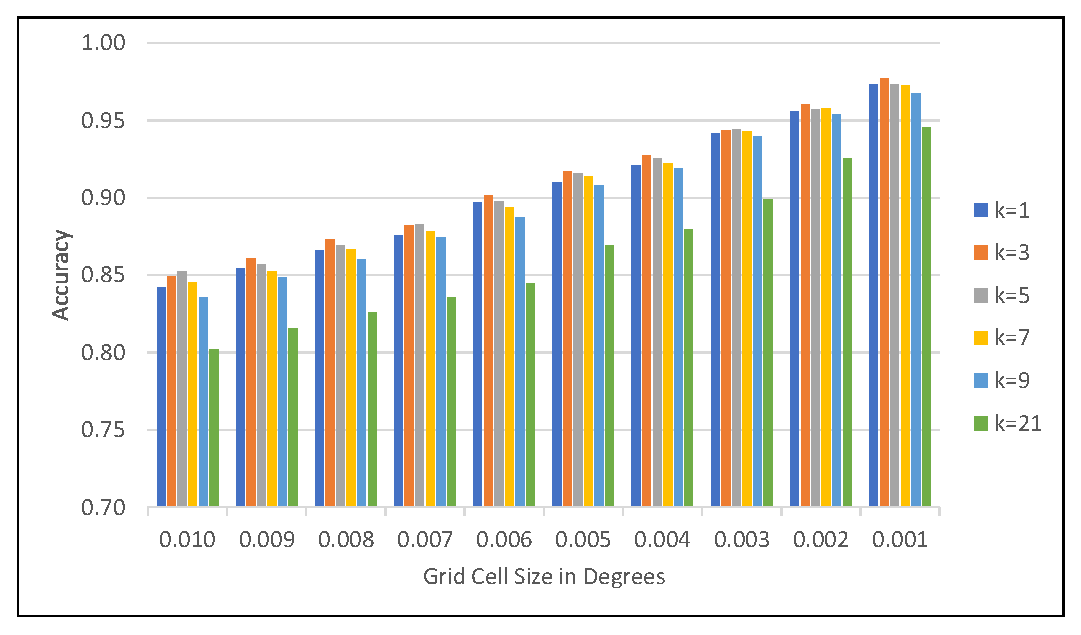
\includegraphics[width = 0.8\textwidth]{figures/jaccard_compare}
		\subcaption{Jaccard Similarity}
    \label{fig:jaccard_compare}
	\end{subfigure}

	\begin{subfigure}[b]{\textwidth}
		\centering
		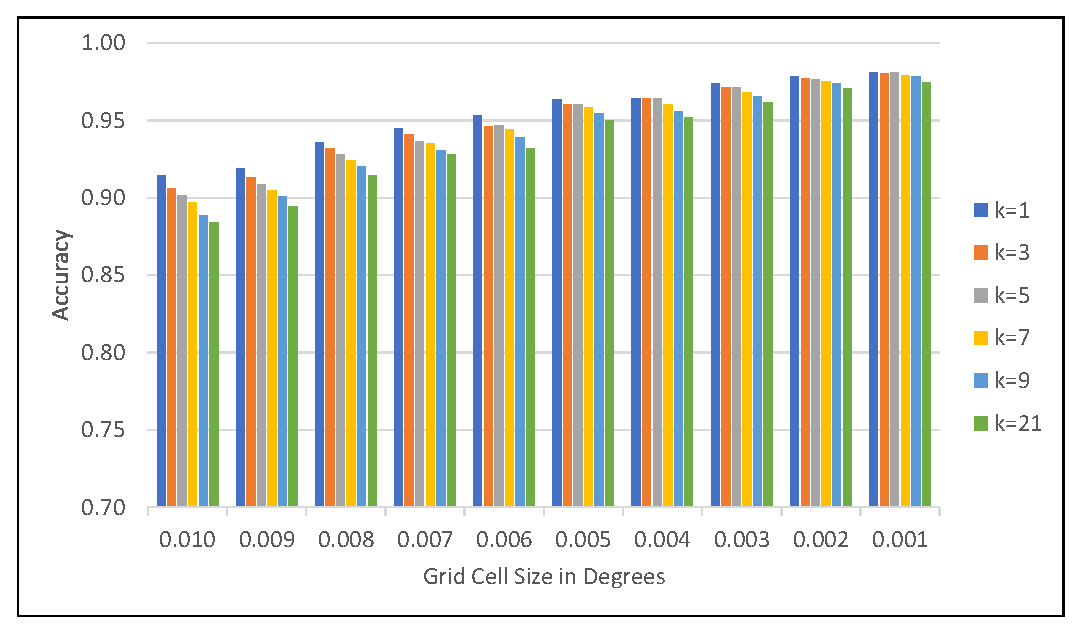
\includegraphics[width = 0.8\textwidth]{figures/cosine_compare}
		\subcaption{Cosine Similarity}
  	\label{fig:cosine_compare}
	\end{subfigure}
  \caption{Classification Accuracy for varying grid-cell size and varying k.}
  \label{fig:results-ext}
	\figSpace
\end{figure}

\section{Accuracy using Set Descriptors}

In the first set of experiments, the accuracy of the user identification is evaluated for different grid-resolutions $ext$, using bitset descriptors for the Jaccard similarity measure (c.f. Definition \ref{subsubsec:set}). The results of this evaluation are shown in Figure \ref{fig:jaccard_compare}. In the basic setting having a relatively coarse spatial grid of $ext=0.01'$, a simple distance weighted $k$NN classification is able to correctly identify up to $85\%$ of individuals for $k=5$. This result improves even further as the grid-resolution $ext$ is increased. In the case of the most detailed grid having $ext=0.001'$, the solution is able to break the $97\%$ classification accuracy line.
This result is quite concerning, as it shows that the motion of individual real-persons is quite characteristic, and that the motion model allows to capture this individuality and allows to discriminate different users very well.

\begin{figure}[tbh]
	\centering
	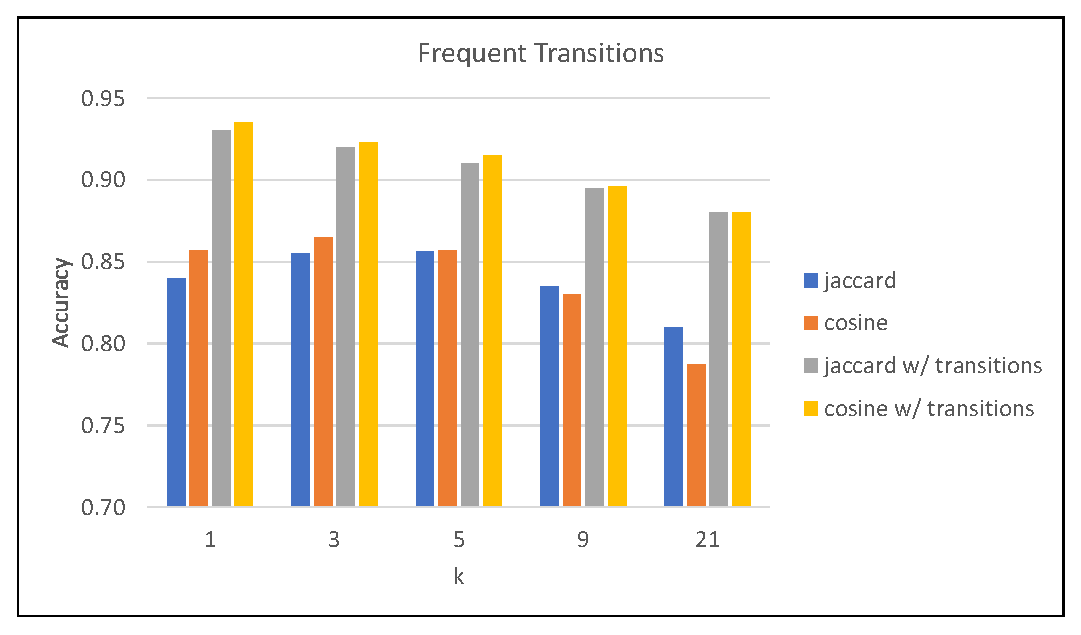
\includegraphics[width = 0.8\textwidth]{figures/topn_transitions}
  \caption{Classification Accuracy using Frequent Transitions.}
  \label{fig:transitions}
	\figSpace
\end{figure}

The classification result are worse for $k=1$ and $k=3$. This result is contributed to chance, as another user may, by chance, have a trajectory very similar to the query trajectory $q_u^e \in Q(u,e)$ of user $u$. However, by using more neighbors, it is likely that the correct user $u$ appears at least twice in the $k=3$ or $k=5$ set, thus out-weighting the erroneous user in the first rank. Yet, for $k>5$ there is a drop in accuracy. This is contributed that the query user only has at most $11$ trajectories in the training set. This number might be less than 11 if a user was not active in all epochs. This is the case for many users, shown by Figure \ref{fig:500_dist}. In the extreme case having $k=21$, at least $10$ trajectories of wrong users must be in the $k$NN result, allowing noise have a much greater effect, especially in the case where $u$ has few trajectories.

Furthermore, Figure \ref{fig:cosine_compare} shows the results using frequency vectors as descriptors, and using the cosine coefficient as a similarity measure (c.f. Definition \ref{subsubsec:set}). The improvement in classification accuracy is relatively minor, but are able to hit the $98\%$ accuracy mark. This result can be contributed to the fact that bitset descriptors already perform so well. Thus, knowing the set of places that a user visited is descriptive enough, such that the frequency of visits does not yield much additional descriptiveness.

\section{Accuracy using Frequent Transitions}

In the next set of experiments, how the usage of transition descriptors (c.f. Section \ref{subsubsec:trans}) instead of set descriptors affects the classification accuracy is evaluated. The results depicted in Figure \ref{fig:transitions} indicate that using from-to-transitions, as opposed to just using sets of cells, further allows to improve the classification quality. An increase in classification accuracy of around $10\%$ (absolute) is observed using transitions, achieving an classification accuracy of nearly $95\%$. This result indicates that the sequence, and thus the motion in space and time is more descriptive than just sets of regions, and thus the motion in space-only.

\section{Accuracy for Different Trajectory Length}
Next, the number of observations required to identify a user accurately is evaluated. Therefore trajectory sizes are created according to the observation distribution in Figure \ref{fig:500_dist}. Then tests are for each trajectory size. If a trajectory does not have the minimum number of observations for the corresponding group, it is not tested, and if a trajectory has more observations than the allowed maximum for the corresponding group, a random sample is taken and tested instead. Thus, instead of testing the accuracy on the original trajectories this tests the accuracy on controlled trajectory sizes.

\begin{figure}[t]
	\centering
	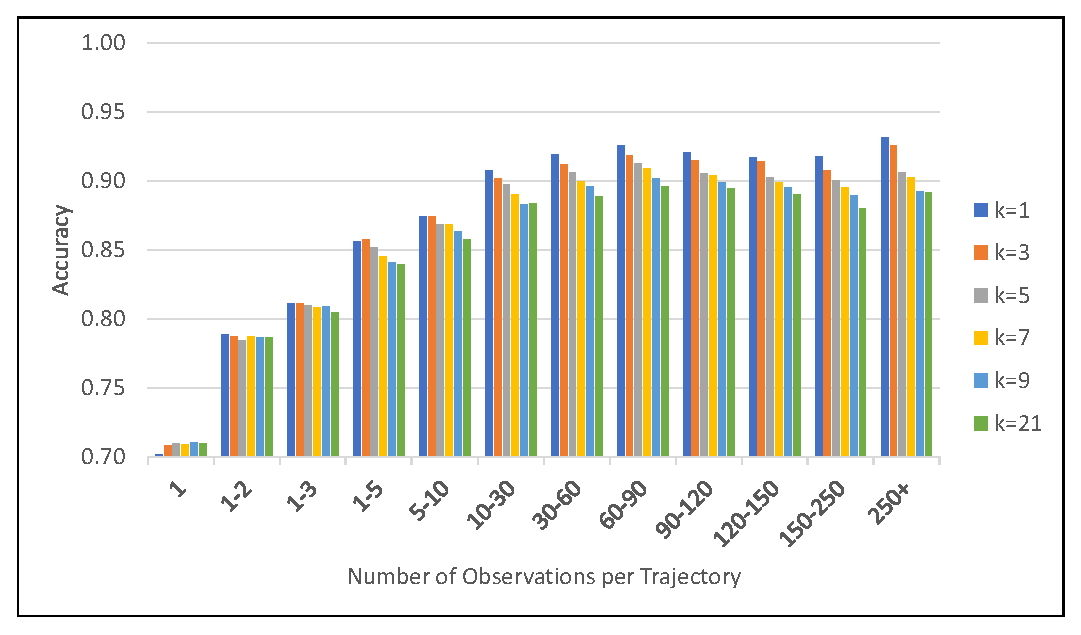
\includegraphics[width = 0.8\textwidth]{figures/archetype_compare}
  \caption{User identification accuracy for different trajectory sizes.}
  \label{fig:archetype}
	\figSpace
\end{figure}

The classification results for each group can be seen in Figure \ref{fig:archetype}. For reference, the set of all trajectories, as used before, is shown first. Surprisingly, in the case of having only one random observation for each trajectory, it is possible to identify over $70\%$ of the users in this dataset. This is likely due to the fact that a random location from a trajectory is likely to pick a users most frequent grid cell, which is most discriminative. Increasing the number of trajectory samples to two, a significant increase in accuracy to $78\%$ is seen, and a steady growth in accuracy from there is shown. Accuracy starts to level off after having 30 or more samples trajectory points from a user. This is surprising, as the vast majority of trajectories has more than 60 observations. Thus, sampling down to 30 observations, yields a significant reduction in data, but as Figure \ref{fig:archetype} shows, yields almost no reduction of discriminative information.

The leveled accuracy level is above $90\%$, which is extremely high for a classification task having 500 different classes. This positive result is also a consequence of large trajectories (i.e., trajectories having a large number of observations) generally having larger trajectories in the training set, as the frequency distribution of tweets among the 500 most prolific Twitter users in London is very skewed. Finally, the classification performs the best, if the parameter of the $kNN$ classification is set to $k=1$. This result is in line with Figure \ref{fig:cosine_compare}, as Cosine-Similarity is used per default in this experiment.

Summarizing this experiment, very short trajectories having $10$ or less observations in space and time are enough to unveil the identity of a user. This is a concerning result.
